\documentclass[xcolor=dvipsnames]{beamer}

\setbeamertemplate{navigation symbols}{}
%\setbeamertemplate{background}[grid][step=1cm]
\useoutertheme{infolines}
\usepackage{graphicx}

\date{}

\begin{document}

\begin{frame}
  \frametitle{3D Field Calculation using Boundary Element Method}

  \begin{columns}
    \begin{column}{0.15\textwidth}
      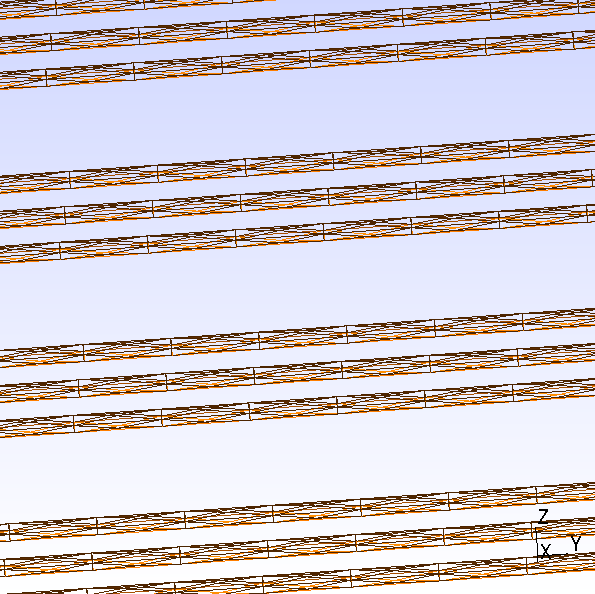
\includegraphics[width=\textwidth]{parallel-mesh.png}      
      
      \tiny fully-parallel wire planes
    \end{column}
    \begin{column}{0.7\textwidth}
      \begin{itemize}\scriptsize
      \item So far just Shockley-Ramo \textit{weighting potentials}.
      \item Meshes with custom code + GMSH and BEM with BEM++.
      \item Fully-parallel wires for checking with prior Garfield 2D.
      \item Initial, full-3D using a MicroBooNE-like geometry.
      \item To do: drift field, ray tracing, average response functions.
      \item BEM seems to perform well as alternative to FEM.
      \end{itemize}
    \end{column}
    \begin{column}{0.15\textwidth}
      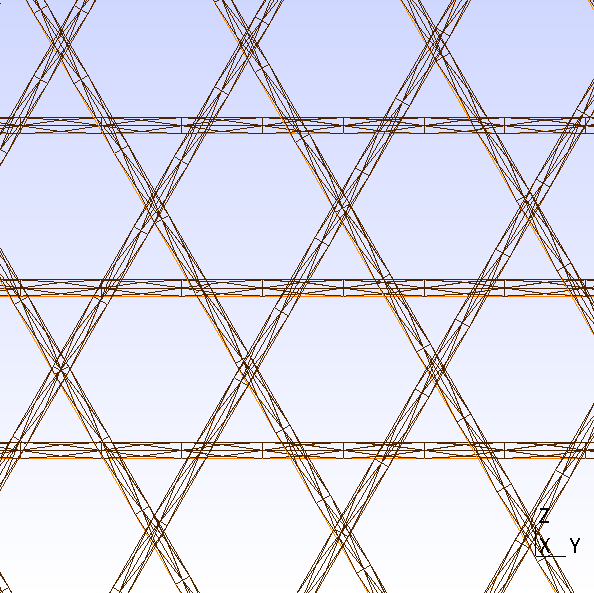
\includegraphics[width=\textwidth]{uboone-mesh.png}

      \tiny MicroBooNE-like geometry
    \end{column}
  \end{columns}

  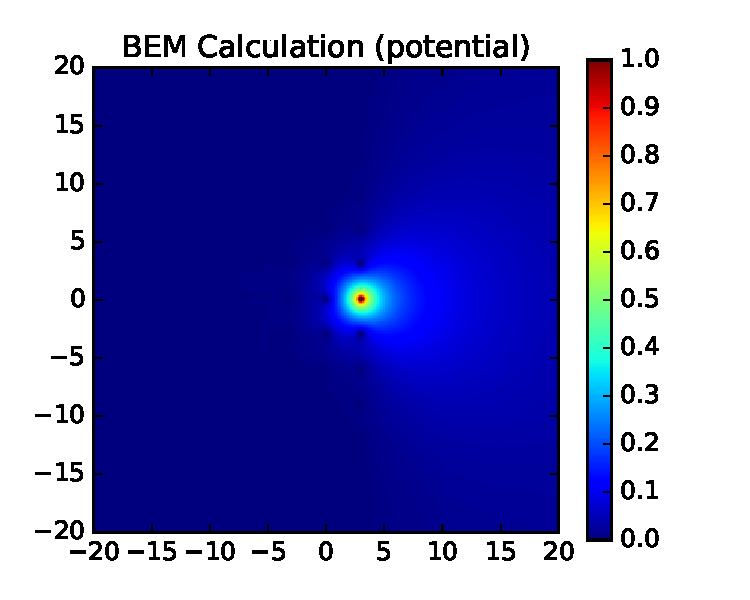
\includegraphics[width=6cm]{parallel-near-d11.pdf}%
  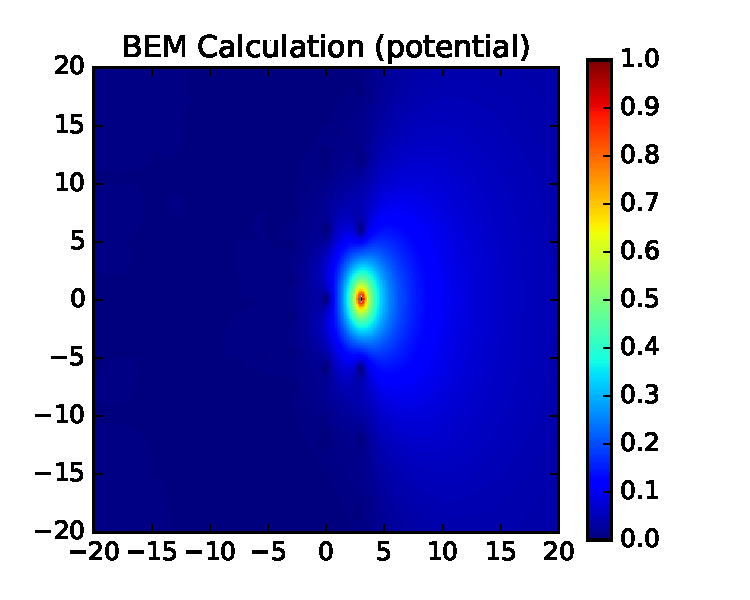
\includegraphics[width=6cm]{uboone-near-d11.pdf}

  \vspace{-3mm}
  \begin{center}\scriptsize
    Weighting potentials, units are mm.
  \end{center}

\end{frame}

\end{document}